\subsubsection{3D convection with an Earth-like initial condition}
\label{sec:cookbooks-S20RTS}
\textit{This section was contributed by Jacqueline Austermann}

For any model run with \aspect{} we have to choose an initial condition for the
temperature field. If we want to model convection in the Earth's mantle we want
to choose an initial temperature distribution that captures the Earth's buoyancy
structure. In this cookbook we present how to use temperature perturbations
based on the shear wave velocity model S20RTS \cite{S20RTS} to
initialize a mantle convection calculation.

\paragraph{The input shear wave model.}

The current version of \aspect{} can read in the shear wave velocity models
S20RTS \cite{S20RTS} and S40RTS \cite{S40RTS}, which are located
in \url{data/initial-temperature/S40RTS/}. Those models provide
spherical harmonic coefficients up do degree 20 and 40, respectively, for 21
depth layers. The interpolation with depth is done through a cubic spline
interpolation. The input files \texttt{S20RTS.sph} and \texttt{S40RTS.sph} were
downloaded from \url{http://www.earth.lsa.umich.edu/~jritsema/Research.html}
and have the following format (this example is S20RTS):

\lstinputlisting[language=prmfile]{cookbooks/initial-condition-S20RTS/doc/S20RTS.input.sph}

The first number in the first line denotes the maximum degree. This is followed in
the next line by the spherical harmonic coefficients from the surface down to the
CMB. The coefficients are arranged in the following way:\\

\noindent $a_{00}$ \\
$a_{10}$ $a_{11}$ $b_{11}$ \\
$a_{20}$ $a_{21}$ $b_{21}$ $a_{22}$ $b_{22}$ \\
... \\

$a_{yz}$ is the cosine coefficient of degree $y$ and order $z$; $b_{yz}$ is
the sine coefficient of degree $y$ and order $z$. The depth layers are specified
in the file \texttt{Spline\_knots.txt} by a normalized depth value ranging from the CMB (3480km,
normalized to -1) to the Moho (6346km, normalized to 1). This is the original
format provided on the homepage.

Any other perturbation model in this same format can also be used, one only
has to specify the different filename in the parameter file (see next section).
For models with different depth layers one has to adjust the \texttt{Spline\_knots.txt}
file as well as the number of depth layers, which is hard coded in the current
code. A further note of caution when switching to a different input model
concerns the normalization of the spherical harmonics, which might differ.
After reading in the shear wave velocity perturbation one has several options
to scale this into temperature differences, which are then used to initialize
the temperature field. It should be noted that the shear wave velocity perturbations in
S20RTS and S40RTS are expressed in terms of percentage deviation from PREM. Wavespeed perturbations
in other models may be referenced to other absolute values and this should be taken into account
when interpreting absolute values of temperature, density and other physical parameters in ASPECT.

\paragraph{Setting up the \aspect{} model.}

For this cookbook we will use the parameter file provided in
\url{cookbooks/initial-condition-S20RTS/S20RTS.prm}, which uses a 3d spherical shell
geometry similar to section \ref{sec:shell-simple-3d}. This plugin is only sensible
for a 3D spherical shell with Earth-like dimensions.

The relevant section in the input file is as follows:

\lstinputlisting[language=prmfile]{cookbooks/initial-condition-S20RTS/doc/S20RTS.part.prm.out}

For this initial condition model we need to first specify the data directory in which
the input files are located as well as the initial condition file (S20RTS.sph or
S40RTS.sph) and the file that contains the normalized depth layers (Spline knots depth file name).
We next have the option to remove the degree 0 perturbation from the shear
wave model. This might be the case if we want to make sure that the depth
average temperature follows the background (adiabatic or constant) temperature.

The next input parameters describe the scaling from the shear wave velocity
perturbation to the final temperature field. The shear wave velocity perturbation
$\delta v_s / v_s$ (that is provided by S20RTS) is scaled into a density perturbation $\delta \rho / \rho$ with a
constant that is specified in the initial condition section of the input parameter
file as `Vs to density scaling'. Here we choose a constant scaling of 0.15. This
perturbation is further translated into a temperature difference $\Delta T$ by
multiplying it by the negative inverse of thermal expansion, which is also
specified in this section of the parameter file as `Thermal expansion coefficient
in initial temperature scaling'. This temperature difference is then added to the
background temperature, which is the adiabatic temperature for a compressible
model or the reference temperature (as specified in this section of the parameter file) for an
incompressible model. Features in the upper mantle such as cratons might
be chemically buoyant and therefore isostatically compensated, in which case
their shear wave perturbation would not contribute buoyancy variations. We therefore included an
additional option to zero out temperature perturbations within a certain depth, however, in this example we don't make use of this functionality. The chemical variation within the mantle
might require a more sophisticated `Vs to density' scaling that varies for
example with depth or as a function of the perturbation itself, which is not captured
in this model. The described procedure
provides an absolute temperature for every point, which will only be adjusted
at the boundaries if indicated in the Boundary temperature model. In this example
we chose a surface and core mantle boundary temperature that differ from the
reference mantle temperature in order to approximate thermal boundary layers.

\paragraph{Visualizing 3D models.}

In this cookbook we calculate the instantaneous solution to examine the flow
field. Figures~\ref{fig:ic-1} and \ref{fig:ic-2} show some of the output
for a resolution of 2 global refinement steps (\ref{fig:ic-1}c and
\ref{fig:ic-2}a, c, e) as used in the cookbook, as well as 4 global
refinement steps (other panels in these figures). Computations with 4 global
refinements are expensive, and consequently this is not the
default for this cookbook. For example, as of 2017, it takes 64 cores approximately
2 hours of walltime to finish this cookbook with 4 global refinements.
Figure~\ref{fig:ic-1}a and b shows the density variation
that has been obtained from scaling S20RTS in the way described above.
One can see the two large low shear wave velocity provinces
underneath Africa and the Pacific that lead to upwelling if they are assumed to
be buoyant (as is done in this case). One can also see the subducting slabs
underneath South America and the Philippine region that lead to local downwelling.
Figure~\ref{fig:ic-1}c and d shows the heat flux density at the surface for
2 refinement steps (c, colorbar ranges from 13 to 19 mW/$m^2$) and for
4 refinement steps (d, colorbar ranges from 35 to 95 mW/$m^2$). A first order correlation
with upper mantle features such as high heat flow at mid ocean ridges and low
heat flow at cratons is correctly initialized by the tomography model.
The mantle flow and buoyancy variations produce dynamic topography on the
top and bottom surface, which is shown for 2 refinement steps (\ref{fig:ic-2}a and c, respectively)
and 4 refinement steps (\ref{fig:ic-2}b and d, respectively).
One can see that subduction zones are visible as depressed surface topography
due to the downward flow, while regions such as Iceland, Hawaii, or mid ocean
ridges are elevated due to (deep and) shallow upward flow. The core mantle boundary
topography shows that the upwelling large low shear wave velocity
provinces deflect the core mantle boundary up. Figure~\ref{fig:ic-2}e and
f shows geoid perturbations for 2 and 4 global refinement steps, respectively.
The geoid anomalies show a strong correlation with the surface dynamic topography.
This is in part expected given that the geoid anomalies are driven by the
deflection of the upper and lower surface
as well as internal density variations. The relative importance of these different
contributors is dictated by the Earth's viscosity profile. Due to the isoviscous
assumption in this cookbook, we don't properly recover patterns of the observed
geoid. Lastly, Figure~\ref{fig:ic-2}g and h shows geoid perturbations for 2 and 4
global refinement steps, respectively.

As discussed in the previous cookbook, dynamic topography does not necessarily
average to zero if the resolution is not high enough. While one can simply subtract
the mean as a postprocessing step this should be done with caution since a non-zero
mean indicates that the refinement is not sufficiently high to resolve the
convective flow. In Figure~\ref{fig:ic-2}a-d we refrained from subtracting the mean but
indicated it at the bottom left of each panel. The mean dynamic
topography approaches zero for increasing refinement. Furthermore, the mean bottom
dynamic topography is closer to zero than the mean top dynamic topography. This is
likely due to the larger magnitude of dynamic topography at the surface and the
difference in resolution between the top and bottom domain
(for a given refinement, the resolution at the core mantle boundary is
higher than the resolution at the surface). The average geoid height and gravity anomaly
is zero since the minimum degree in the geoid anomaly expansion is set to 2.

This model uses a highly simplified material model that is incompressible and
isoviscous and does therefore not represent real mantle flow. More realistic
material properties, density scaling as well as boundary conditions will affect the magnitudes
and patterns shown here. A comparison between surface dynamic topography, the geoid,
and gravity anomalies from ASPECT and a spectral based code shows good agreement
(see \texttt{benchmarks/spectral-comparison/} for figure and details).

\begin{figure}
  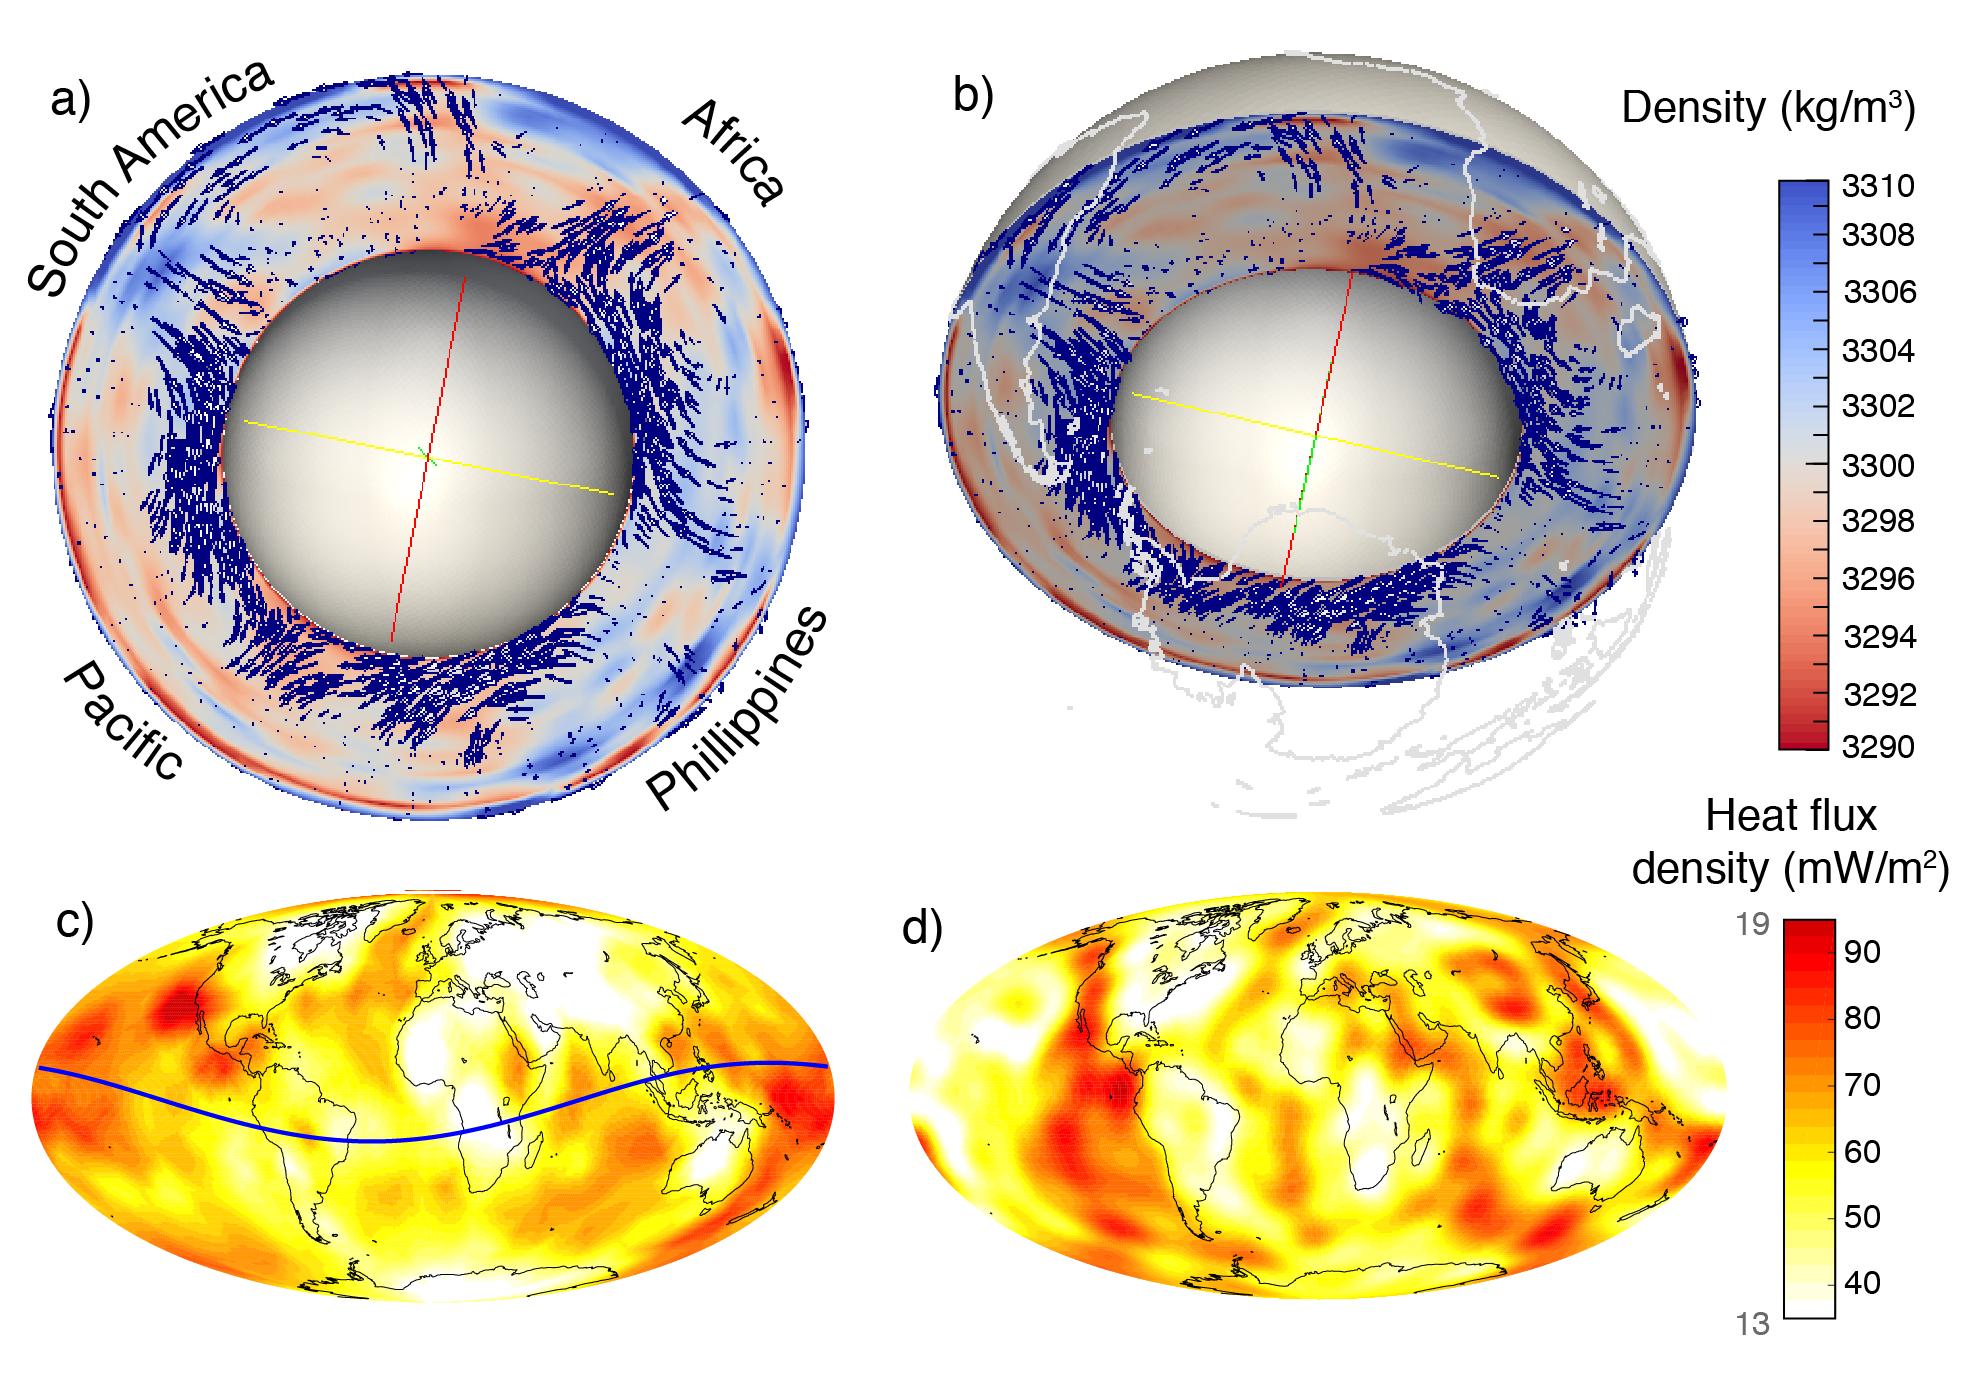
\includegraphics[width=\textwidth]{cookbooks/initial-condition-S20RTS/doc/Fig_cookbook_V4-01.png}
  \hfill
  \caption{\it Panels (a) and (b) show the density distribution as prescribed from the shear
  wave velocity model S20RTS and the resulting flow for a global refinement of 4. This
  model assumes a constant scaling between shear wave and density perturbations.
  Panel (c) shows the great circle (dashed blue line) along which the top slices
  are evaluated. Panels (c) and (d) show the resulting heat flux density for a global refinement of
  2 (c, cookbook) and 4 (d). The colorbar ranges from 13 to 19 mW/$m^2$ for panel (c) and
  from 35 to 95 mW/$m^2$ for panel (d).}
  \label{fig:ic-1}
\end{figure}

\begin{figure}
  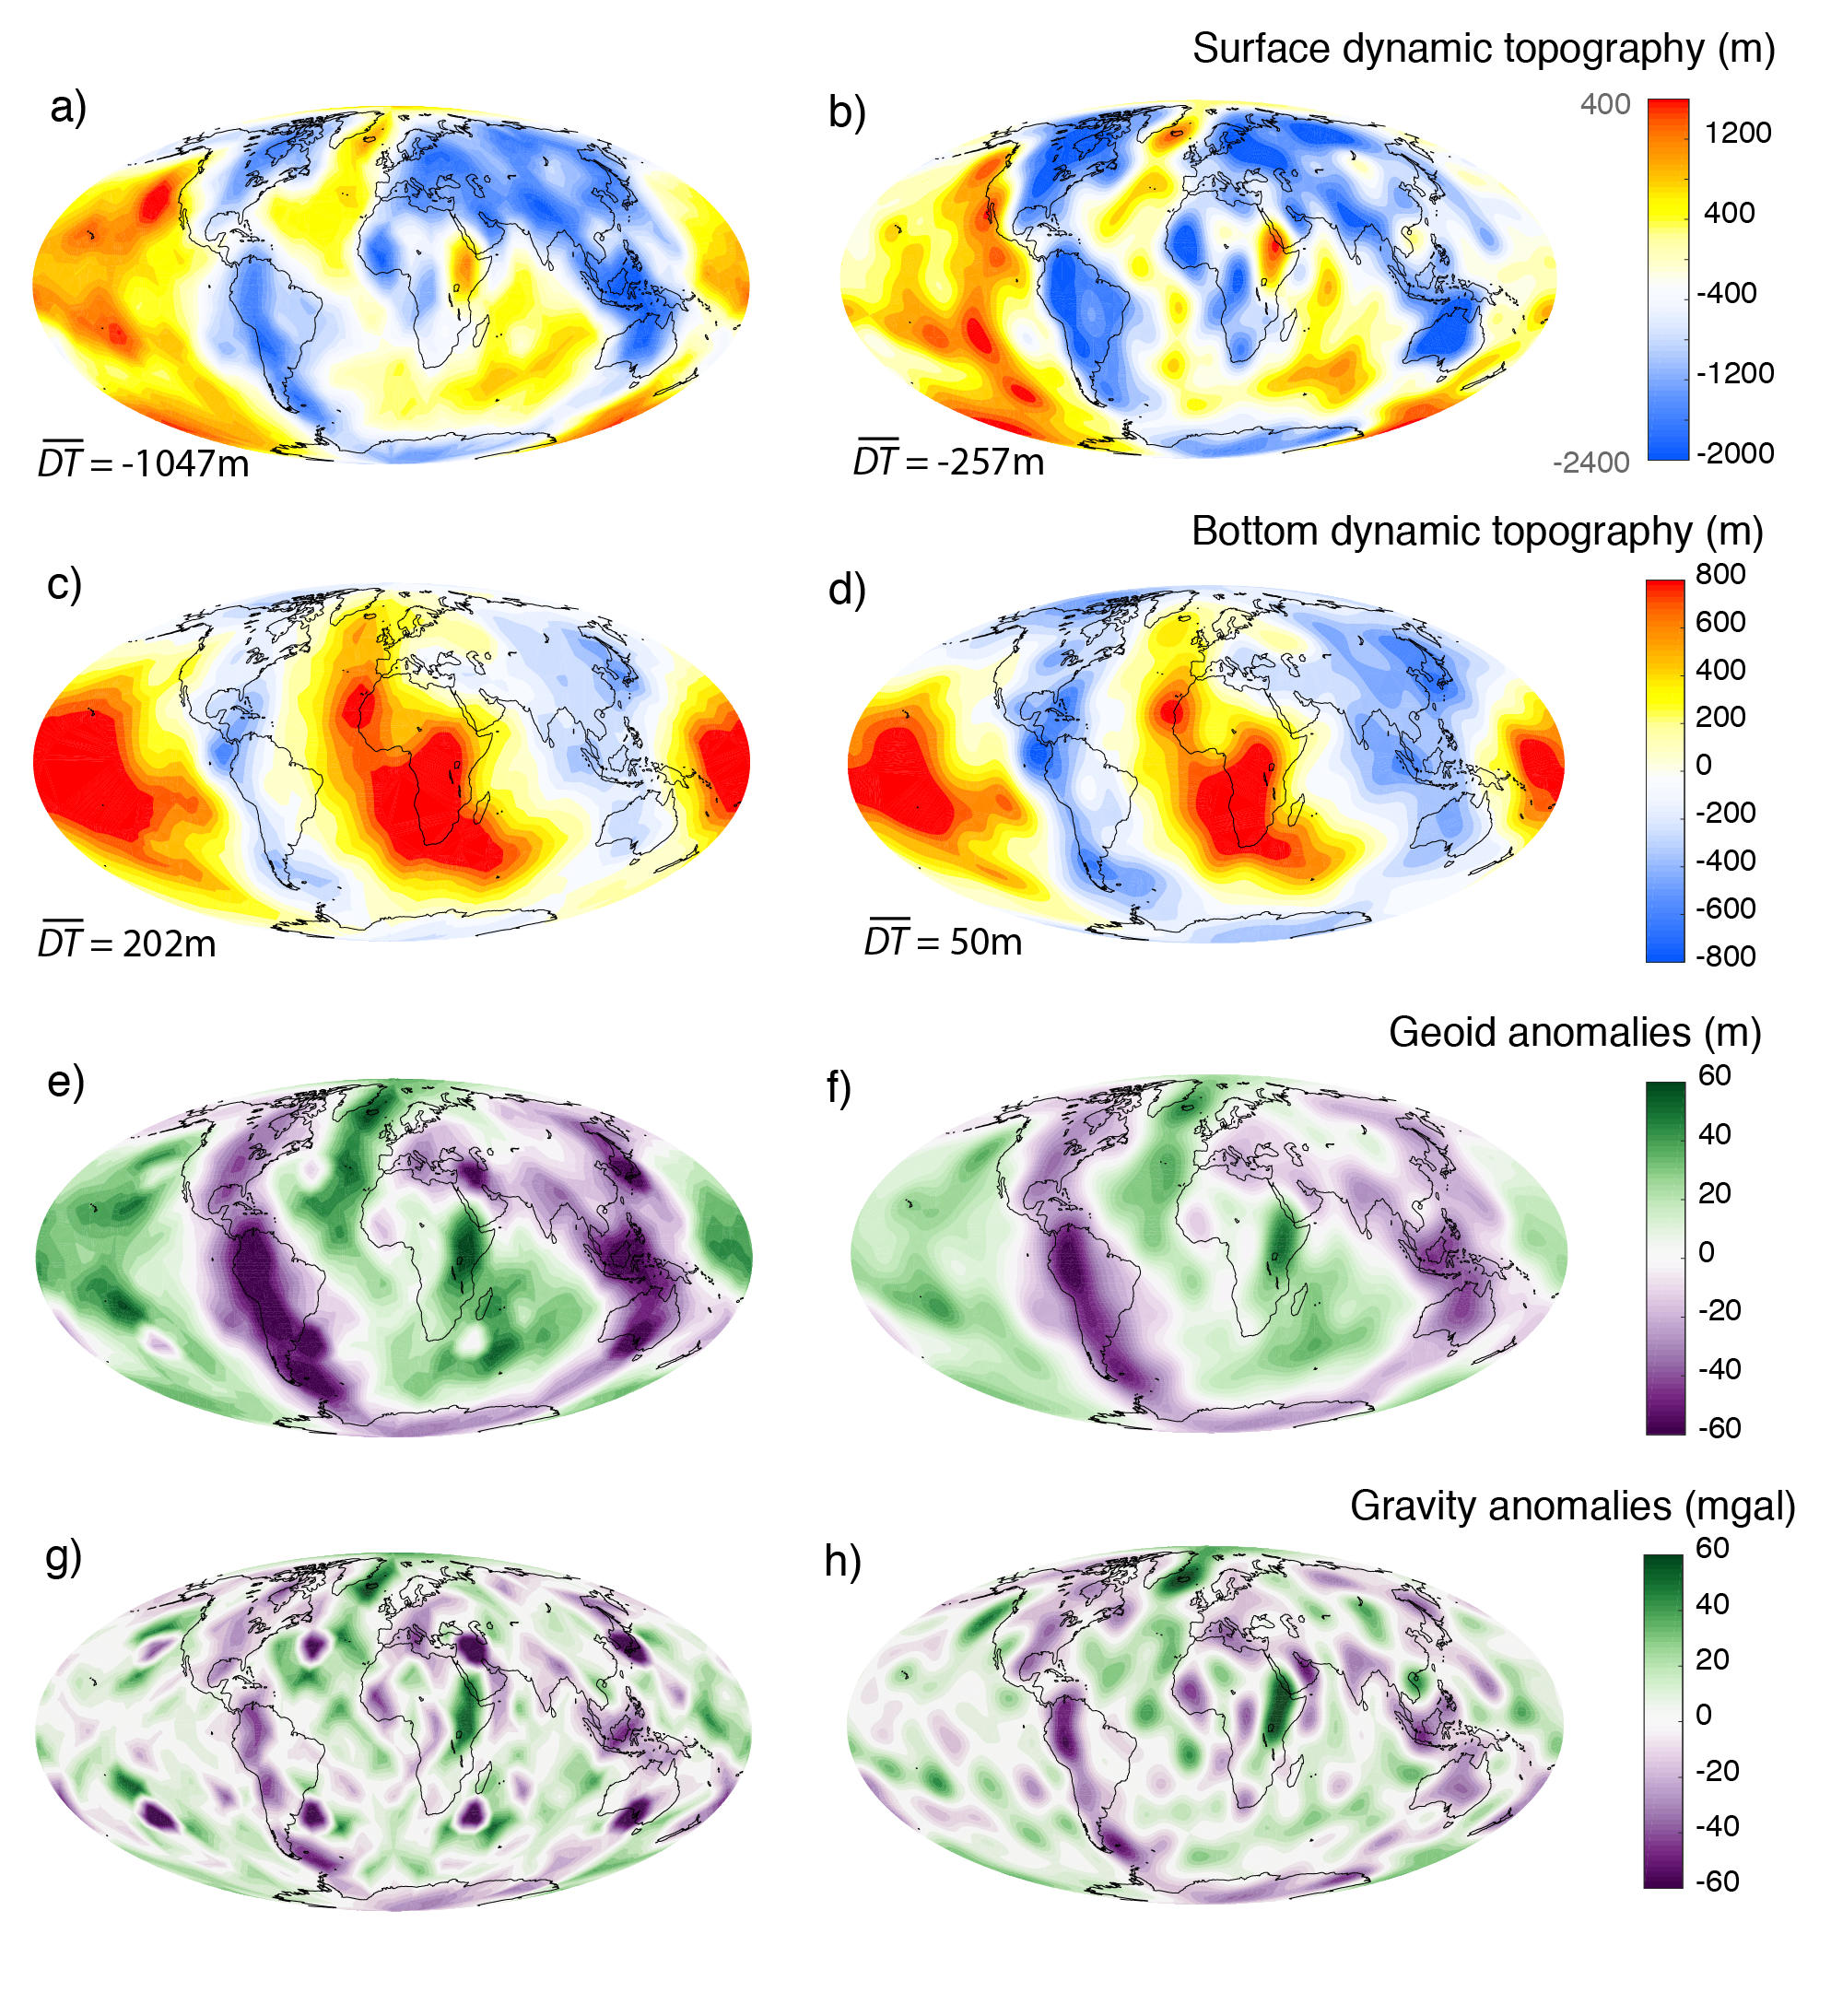
\includegraphics[width=\textwidth]{cookbooks/initial-condition-S20RTS/doc/Fig_cookbook_V4-02.png}
  \hfill
  \caption{\it The first row of this figure shows the surface dynamic topography resulting
  from the flow shown in Figure~\ref{fig:ic-1} for a global
  refinement of 2 (a, cookbook) and 4 (b). The colorbar ranges from -2400m to 400m for panel (a) and
  from -2000m to 1600m for panel (b). The second row shows the dynamic topography at
  the core mantle boundary for the same model and a refinement of 2 (c, cookbook) and 4 (d). Averages of the
  dynamic topography fields are indicated at the bottom left of each panel. The third row shows the
  geoid anomalies from this model at the surface for refinement of 2 (e, cookbook) and 4 (f).
  The fourth row shows the gravity anomalies from this model at the surface for refinement of 2
  (g, cookbook) and 4 (h)}
  \label{fig:ic-2}
\end{figure}


